% Drawing 154/03-14 -- folder 154, batch 03, archive page 50 (PDF page 51).
% Transcription: figures à la suite de b) : un segment vert barré de rouge et d'orange, biffé ; au-dessous, un segment vert en pointillé portant en son milieu un trait rouge épais barré d'une petite croix ; à droite, un coin vert (une branche en pointillé, puis pleine), un point rouge sur chaque branche et un trait orange au coin
% Kind: three small figures (one struck). Method 2 (schematic redraw from the facsimile). Status: ok.
% Notes: The first figure (a green segment barred with red and orange) is struck out with a pen scribble and is not drawn. Drawn: the dotted green segment with a thick red piece in its middle crossed by a short orange-red tick; the green corner, its upper branch dotted then solid, a red point on it, the horizontal branch with a red point, a short orange stroke across the corner. Redrawn 2026-11-12 (issue 128): to check again.
% Coordinates: 1 unit = 1 mm = 1/100 of the crop width (bbox in page fractions: [0.24, 0.315, 0.5, 0.37]).
% Redrawn by Claude (claude-fable-5-2), issue #128, 2026-11-12; not checked by a human; not compiled (no TeX in the session).
% Rights: reproduces part of the work -- behind RENDER_TRANSCRIPTS, never published by itself.
\documentclass[tikz,border=3pt]{standalone}
\usepackage{amsmath,amssymb}
\usetikzlibrary{patterns,arrows.meta}
\tikzset{Or/.style={orange!90!black}, Lg/.style={green!60!black!70}, Rd/.style={red!85!black}, pencil/.style={black!45}, struck/.style={black!35}, mpt/.style={circle,draw,inner sep=1.3pt}, pt/.style={circle,fill,inner sep=0.9pt}, opt/.style={circle,draw,fill=white,inner sep=1.1pt}}
\begin{document}
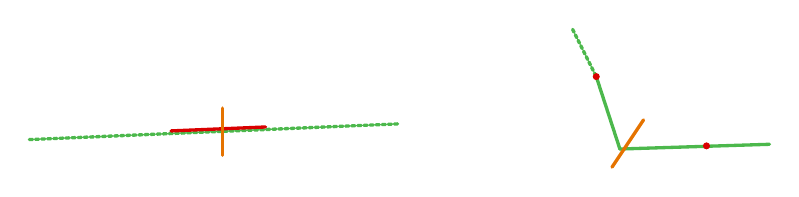
\begin{tikzpicture}[x=1mm,y=1mm,line cap=round,line join=round,font=\scriptsize]
\draw[Lg,densely dotted,very thick] (3,-24) -- (50,-22);
\draw[Rd,very thick] (21,-22.9) -- (33,-22.4);
\draw[Or,very thick] (27.5,-20) -- (27.5,-26);
\draw[Lg,densely dotted,very thick] (72,-10) -- (75,-16);
\draw[Lg,very thick] (75,-16) -- (78,-25.2);
\draw[Lg,very thick] (78,-25.2) -- (97,-24.6);
\node[pt,Rd] at (75,-16) {};
\node[pt,Rd] at (89,-24.8) {};
\draw[Or,very thick] (77,-27.5) -- (81,-21.5);
\end{tikzpicture}
\end{document}
